\section{Objetivo}
Que el alumno implemente una clase \classname{Factor} para familiarizarse con las operaciones entre factores que se utilizan para realizar inferencia en redes Bayesianas

\section{Introducción}

\quotes{Sea \(D\) un conjunto de variables aleatorias. Se define un Factor $\phi$ como una función de \(Val(D)\) a \(\mathbb{R}\). Un factor es no-negativo si todas sus entradas son no negativas. Al conjunto de variables \(D\) se le llama \textit{alcance del factor} y se denota como \(Alcance(\phi)\) } \parencite[104]{KollerFriedman2009}.

Tomando como base la definición de Koller Y Friedman, la Dra. Verónica define a un Factor como \quotes{Una estructura matemática definida sobre un conjunto de variables donde cada variable puede tomar valores de su dominio. A este conjunto de variables se les denomina como el alcance del factor; el factor asocia un número real a cada posible asignación de valores de esas variables}. Es importante notar que, debido a la misma definición del Factor, el resultado de cada operación entre factores no siempre será una medida de probabilidad, como lo podemos ver en la figura~\ref{fig:FactorABC}.

En cuanto a las operaciones de Factores que se explicarán en esta práctica, nos basamos en las operaciones que presentan Koller Y Friedman y que se utilizan en la materia: multiplicación, reducción, marginalización y normalización. 

\subsection[Operaciones]{Operaciones entre Factores}

\subsubsection{Multiplicación}
\quotes{Sean $X$, $Y$ y $Z$ tres conjuntos disjuntos de variables aleatorias, y sean $\phi_1(X,Y)$ y $\phi_2(Y,Z)$ dos factores. Se define el Factor producto $\phi_1(X,Y) \times \phi_2(Y,Z)$ como un factor $\psi: Val(X,Y,Z) \mapsto \mathbb(R)$ de la siguiente forma: \[ \psi(X,Y,Z) = \phi_1(X,Y) \cdot \phi_2(Y,Z)\]} \parencite[107]{KollerFriedman2009}.

La operación de multiplicación es un poco sencilla. Si los conjuntos de variables de los factores a multiplicar no tienen elementos en común, se multiplica cada entrada del factor A por cada entrada del Factor B. El alcance del factor resultante es la unión de los alcances de los factores a multiplicar \parencite[107]{KollerFriedman2009}. Por ejemplo: Tenemos tres factores A, B y C,


\begin{figure}[h!]
    \centering
    \begin{subfigure}[b]{0.3\textwidth}
        \centering
        \begin{tabular}{ l | r }
          A & $\phi$(A)\\ \hline
          0 & .3  \\ \hline
          1 & .7  \\
        \end{tabular}
        \caption{Factor A}
    \end{subfigure}
    ~ 
    \begin{subfigure}[b]{0.3\textwidth}
        \centering
        \begin{tabular}{ l | r }
          B & $\phi$(B)\\ \hline
          0 & .6  \\ \hline
          1 & .4  \\
        \end{tabular}
        \caption{Factor B}
    \end{subfigure}
    ~
    \begin{subfigure}[b]{0.3\textwidth}
        \centering
        \begin{tabular}{ l | r }
          C & $\phi$(C)\\ \hline
          0 & .2  \\ \hline
          1 & .8  \\
        \end{tabular}
        \caption{Factor C}
    \end{subfigure}
\end{figure}

\noindent Para obtener el factor AB, se multiplicaría el renglón A=0 con B=0, luego A=0 con B=1, A=1 con B=0 y por último A=1 con B=1:

\begin{figure}[H]
  \begin{center}
    \begin{tabular}{ l  c | r }
      A & B & $\phi$(A,B)\\ \hline
      0 & 0 & (.3)*(.6)  \\ \hline
      0 & 1 & (.3)*(.4)  \\ \hline
      1 & 0 & (.7)*(.6)  \\ \hline
      1 & 1 & (.7)*(.4)  \\
    \end{tabular}
  \end{center}
  \caption{Factor AB}
  % \label{fig:FactorA}
\end{figure}

\noindent Si el alcance de ambos factores tiene variables en común, se debe asegurar que tengan el mismo valor en cada renglón por multiplicar. Por ejemplo, si se tienen los factores AB y AC, al momento de multiplicar el renglón \{A=0,B=0\} se debe seleccionar los renglones donde A=0 en el factor AC, estos son \{A=0,C=0\} y \{A=0,C=1\}:

\begin{figure}[h!]
    \centering
    \begin{subfigure}[b]{0.4\textwidth}
        \centering
        \begin{tabular}{ l  c | r }
          A & B & $\phi$(A,B)\\ \hline
          0 & 0 & (.3)*(.6)  \\ \hline
          0 & 1 & (.3)*(.4)  \\ \hline
          1 & 0 & (.7)*(.6)  \\ \hline
          1 & 1 & (.7)*(.4)  \\
        \end{tabular}
        \caption{Factor AB}
    \end{subfigure}
    ~ 
    \begin{subfigure}[b]{0.4\textwidth}
        \centering
        \begin{tabular}{ l  c | r }
          A & C & $\phi$(A,C)\\ \hline
          0 & 0 & (.3)*(.2)  \\ \hline
          0 & 1 & (.3)*(.8)  \\ \hline
          1 & 0 & (.7)*(.2)  \\ \hline
          1 & 1 & (.7)*(.8)  \\
        \end{tabular}
        \caption{Factor AC}
    \end{subfigure}
\end{figure}


\begin{figure}[H]
  \begin{center}
    \begin{tabular}{ l  l  c | r }
      A & B & C & $\phi$(A,B,C)\\ \hline
      0 & 0 & 0 & [(.3)*(.6)]*[(.3)*(.2)]  \\ \hline
      0 & 0 & 1 & [(.3)*(.6)]*[(.3)*(.8)]  \\ \hline
      0 & 1 & 0 & [(.3)*(.4)]*[(.3)*(.2)]  \\ \hline
      0 & 1 & 1 & [(.3)*(.4)]*[(.3)*(.8)]  \\ \hline
      1 & 0 & 0 & [(.7)*(.6)]*[(.7)*(.2)]  \\ \hline
      1 & 0 & 1 & [(.7)*(.6)]*[(.7)*(.8)]  \\ \hline
      1 & 1 & 0 & [(.7)*(.4)]*[(.7)*(.2)]  \\ \hline
      1 & 1 & 1 & [(.7)*(.4)]*[(.7)*(.8)]  \\ 
    \end{tabular}
  \end{center}
  \caption{Factor ABC}
  \label{fig:FactorABC}
\end{figure}

Es importante hacer notar que al multiplicar los factores AB y AC no se estaría obteniendo la probabilidad conjunta de A, B y C, si no alguna otra función $$\phi(A,B,C)$$. 

\subsubsection{Reducción}
\quotes{Sea $\phi(Y)$ un factor y \(U = u\) una asignación para \(U \subseteq Y\). Se define la reducción de un factor $\phi$ al contexto \(U = u\), denotado como \(\phi[U = u]\) (y abreviado como $\phi[u]$), como un factor con alcance \(Y' = Y - U\) de tal forma que \[\phi[u](y') = \phi(y',u)\]} \parencite[111]{KollerFriedman2009}.

La operación de reducción consiste en tomar un valor de alguna variable del factor y sólo tomar los renglones que cumplen con el valor dado de la variable. Por ejemplo: Se tiene el factor AB,

\begin{figure}[H]
  \begin{center}
    \begin{tabular}{ l  c | r }
      A & B & $\phi$(A,B)\\ \hline
      0 & 0 & .18  \\ \hline
      0 & 1 & .12  \\ \hline
      1 & 0 & .42  \\ \hline
      1 & 1 & .28  \\
    \end{tabular}
  \end{center}
  \caption{Factor AB}
  % \label{fig:FactorA}
\end{figure}

\noindent Si se desea reducir con A = 0, el resultado sería un factor:

\begin{figure}[h]
  \begin{center}
    \begin{tabular}{ l | r }
      B & \(\phi(B)\)\\ \hline
      0 & .18  \\ \hline
      1 & .12  \\
    \end{tabular}
  \end{center}
  \caption{Factor \(B\)}
  % \label{fig:FactorA}
\end{figure}

\subsubsection{Normalización}
Para normalizar un factor, esto es, que los valores que toma el factor sumen 1, basta con sumar todos los valores asociados a las asignaciones y dividir cada uno entre esta suma. Por ejemplo: Tenemos el factor \(\phi(B)\), la suma de sus posibles valores es .3, entonces tendríamos:

% TODO: Cambiar por un factor de probabilidad conjunta, donde no sumen uno sus renglones
\begin{figure}[H]
  \begin{center}
    \begin{tabular}{ l  c | r }
      A & B &  \(\phi(B)\)\\ \hline
      0 & 0 & (.18/.3)= .6  \\ \hline
      0 & 1 & (.12/.3)= .4 \\
    \end{tabular}
  \end{center}
  \caption{Factor \(B\)}
  % \label{fig:FactorA}
\end{figure}

% \noindent Esta operación es útil cuando se desea calcular probabilidades condicionales.

\subsubsection{Marginalización}
\quotes{Sea $X$ un conjunto de variables y sea \(Y \notin X\) una variable y $\phi(X,Y)$ un factor. Se define la marginalización de $Y$ en $\phi$, denotado como \(\sum_Y \phi\), como un factor $\psi$ sobre $X$ de tal forma que \[\psi(X) = \sum_Y \phi(X,Y)\]} \parencite[297]{KollerFriedman2009}.

La operación de marginalización consiste en tomar la variable a marginalizar, sumar los valores en los renglones en que cambia su valor pero el de las demás variables no, y asignar esta suma al renglón correspondiente de las variables restantes. Por ejemplo: tenemos el factor AB y deseamos marginalizar la variable B. Entonces, tomamos los renglones donde A=0 y los sumamos, tomamos los renglones donde A=1 y los sumamos:

\begin{figure}[H]
    \centering
    \begin{subfigure}[b]{0.4\textwidth}
        \centering
        \begin{tabular}{ l l  c | r }
           & A & B & $\phi$(A,B)\\ \cline{2-4}
          \(\to\) & 0 & 0 & .18  \\ \cline{2-4}
          \(\to\) & 0 & 1 & .12  \\ \cline{2-4}
           & 1 & 0 & .42  \\ \cline{2-4}
           & 1 & 1 & .28  \\
        \end{tabular}
        \caption{Factor AB}
    \end{subfigure}
    ~ 
    \begin{subfigure}[b]{0.4\textwidth}
        \centering
        \begin{tabular}{l  l | r }
            & A & $\phi$(A)\\ \cline{2-3}
        \(\to\) & 0 & (.18)+(.12)  \\
        \end{tabular}
        \caption{Factor A}
    \end{subfigure}
    \caption{Paso 1}
\end{figure}

% \noindent y

\begin{figure}[H]
    \centering
    \begin{subfigure}[b]{0.4\textwidth}
        \centering
        \begin{tabular}{ l l  c | r }
           & A & B & $\phi$(A,B)\\ \cline{2-4}
           & 0 & 0 & .18  \\ \cline{2-4}
           & 0 & 1 & .12  \\ \cline{2-4}
          \(\to\) & 1 & 0 & .42  \\ \cline{2-4}
          \(\to\) & 1 & 1 & .28  \\
        \end{tabular}
        \caption{Factor AB}
    \end{subfigure}
    ~ 
    \begin{subfigure}[b]{0.4\textwidth}
        \centering
        \begin{tabular}{l  l | r }
            & A & $\phi$(A)\\ \cline{2-3}
            & 0 & (.18)+(.12)  \\ \cline{2-3}
        \(\to\) & 1 & (.42)+(.28)  \\
        \end{tabular}
        \caption{Factor A}
    \end{subfigure}
    \caption{Paso 2}
\end{figure}


\subsection{Desarrollo e implementaci\'on}

\noindent La práctica consiste en crear una clase \classname{Factor} que implemente la operaciones de multiplicación, reducción y normalización de factores y marginalización de variables. Todo esto utilizando el lenguaje de programación \classname{Python}.


\subsubsection{Implementaci\'on}

\begin{enumerate}
  \item Crear una clase \classname{Variable}, con los siguientes atributos: \classname{nombre} y \classname{valores\_posi \linebreak bles} y sobrescribir el método \classname{\_\_str\_\_}.
  % \item Programar un método \classname{tabla\_de\_valores} que reciba como parámetro una lista de objetos tipo \classname{Variable} y que regrese una matriz (lista de listas) que contenga todas las combinaciones de los valores que pueden tomar las variables. TIP: Inicializa la matriz con una única columna que contenga los valores posibles de la primer variable. Después, para cada variable restante, crear una nueva tabla. La nueva tabla es el resultado de anexar los valores posibles de la variable actual por cada renglón de la tabla anterior.
  \item Crear una clase \classname{Factor} que contenga los atributos: 
    \begin{itemize}
      \item \classname{alcance}: una lista de objetos de clase \classname{Variable}.
      \item \classname{valores}: una lista de valores asociados a cada renglón.
      % \item \classname{tabla\_valores}: el resultado del método del paso anterior.
    \end{itemize}
  Deben asegurarse que la lista de valores se encuentre en el orden correspondiente a cada asignación indicada por la tabla de valores del objeto.
  \item Programar un método auxiliar que reciba como parámetro un diccionario con variables y su valor asignado, que obtenga el índice en la tabla de valores que represente esta asignación. Para poder obtener el valor para la asignación de cada variable, deberán utilizar un polinomio de direccionamiento. En general, el polinomio de direccionamiento para un factor de 3 variables se vería así:
      \[(pos(a) * |B| * |C|) + (pos(b) * |C|) + pos(c)\]
    donde \(pos(a)\) es la posición del valor asociado a la variable \(A\) en su lista de valores posibles y \(|A|\) es el tamaño de esta lista. TIP: Pueden factorizar las variables comunes e implementar una   función auxiliar que calcule recursivamente el valor del polinomio de direccionamiento.
  \item Implementa las operaciones: multiplicación, reducción, normalización y marginalización. TIP: Crea primero el factor resultado. Para cada renglón en la tabla de valores de este factor, encuentra los renglones relevantes en los operandos utilizando el método auxiliar mencionado en el punto anterior y realiza la operación correspondiente.
\end{enumerate}

\textbf{\\Entrada} (opcional)\bigskip

\noindent El programa deberá recibir la descripción de los factores en un archivo de texto. A continuación se define la sintaxis del archivo con los factores:

\begin{itemize}
  \item Variables: 
    \begin{align*}
      [&\{<Var_1>:<val_0>, . . . , <val_m>\},\\
      &\{<Var_2>:<val_0>, . . . , <val_m>\}, . . . ,\\
      &\{<Var_n>:<val_0>, . . . , <val_m>\}]
    \end{align*}
    Donde \(<Var_{i}>\) indica el nombre de la variable y \(<val_i>\) los valores que puede tomar la variable.
  \item Factores: 
    \begin{align*}
      [&\{<Var_1>,<Var_2>, . . . , <Var_n> | <Var_{c1}>,<Var_{c2}>, . . ., <Var_{cn}>\},\\
      & . . . , \\
      &\{<Var_1>,<Var_2>, . . . , <Var_n>\}]
    \end{align*}
    Donde \(<Var_{i}>\) indica las variables del factor, \(\mid\) que es un factor condicional y \(<Var_{ci}>\) las variables condicionantes.
  \item Valores: 
    \begin{align*}
      [&\{(Factor_1)_{val1}, (Factor_1)_{val2}, . . . , (Factor_1)_{valk}\},\\
      &\{(Factor_2)_{val1}, (Factor_2)_{val2}, . . . , (Factor_2)_{valk}\},\\
      & . . . \\
      &\{(Factor_j)_{val1}, (Factor_j)_{val2}, . . . , (Factor_j)_{valk}\}]
    \end{align*}
    Donde \((Factor_i)_{valn}\) indica el valor numérico correspondiente a cada renglón del \(Factor_i\). Deben tener en cuenta que se toma la última variable especificada en el renglón de Factores como la que cambia más rápidamente.
\end{itemize}


\noindent Por ejemplo, el archivo:

\begin{minted}[mathescape,
               linenos,
               numbersep=5pt,
               gobble=2,
               frame=lines,
               fontsize=\scriptsize,
               framesep=2mm]{text}
  Variables: [{A : 0, 1}, {B : 0, 1}, {C : 0, 1, 2}]
  Factores: [{A, B}, {A, B, C}]
  Valores: [{0.1, 0.9, 0.5, 0.1}, {0.25, 0.15, 0.35, 0.1, 0.65, 0.8, 0.6, 0.8, .1, .2, .4, .25}]
\end{minted}

\noindent representa los factores:\par

\begin{figure}[H]
    \centering
    \begin{subfigure}[b]{0.4\textwidth}
        \centering
        \begin{tabular}{ l  c | r }
          A & B & $\phi$(A,B)\\ \hline
          0 & 0 & 0.1  \\ \hline
          0 & 1 & 0.9  \\ \hline
          1 & 0 & 0.5  \\ \hline
          1 & 1 & 0.1  \\
        \end{tabular}
        \caption{Factor 1}
    \end{subfigure}
    ~ 
    \begin{subfigure}[b]{0.4\textwidth}
        \centering
        \begin{tabular}{ l l  c | r }
          A & B & C &  \(\phi(A,B,C)\)\\ \hline
          0 & 0 & 0 & 0.25  \\ \hline
          0 & 0 & 1 & 0.15  \\ \hline
          0 & 0 & 2 & 0.35  \\ \hline
          0 & 1 & 0 & 0.1  \\ \hline
          0 & 1 & 1 & 0.65  \\ \hline
          0 & 1 & 2 & 0.8 \\ \hline
          1 & 0 & 0 & 0.6  \\ \hline
          1 & 0 & 1 & 0.8  \\ \hline
          1 & 0 & 2 & 0.1  \\ \hline
          1 & 1 & 0 & 0.2  \\ \hline
          1 & 1 & 1 & 0.4  \\ \hline
          1 & 1 & 2 & 0.25 \\
        \end{tabular}
        \caption{Factor 2}
    \end{subfigure}
    \caption{Factores representados en el archivo}
\end{figure}


\noindent Esta práctica deberá ser implementada usando \classname{Python}.

\section{Requisitos y resultados}

Deberán hacer casos de prueba para marginalización, reducción, normalización y multiplicación de factores. Basta con incluir un pequeño \textit{script} con sus casos de prueba. No es necesario que lo hagan a prueba de todo, no me fijaré en eso.

Para evaluar y calificar la práctica es necesario que se implementen todos los métodos mencionados e indicados, respetando las especificaciones de estilo y documentación del lenguaje de programación que usarán.
Es completamente válido utilizar bibliotecas adicionales si lo consideran necesario, así como la creación y uso de sus propios métodos auxiliares si lo desean.

En la figura~\ref{fig:P5solution} pueden apreciar el resultado de crear 3 factores y ejecutar las operaciones de multiplicación, normalización, reducción y marginalización entre ellos. 

\begin{figure}[H]
  \centering
  \begin{subfigure}[b]{.45\textwidth}
    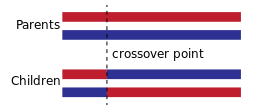
\includegraphics[scale=0.28]{factores/screen1.png}
    \caption{Creación de factores f1 y f2}
  \end{subfigure}
  ~
  \begin{subfigure}[b]{.45\textwidth}
    
\includegraphics[scale=0.28]{factores/screen2.png}
    \caption{Multiplicando f1 y f2, para obtener f3}
  \end{subfigure}


  \begin{subfigure}[b]{.45\textwidth}
    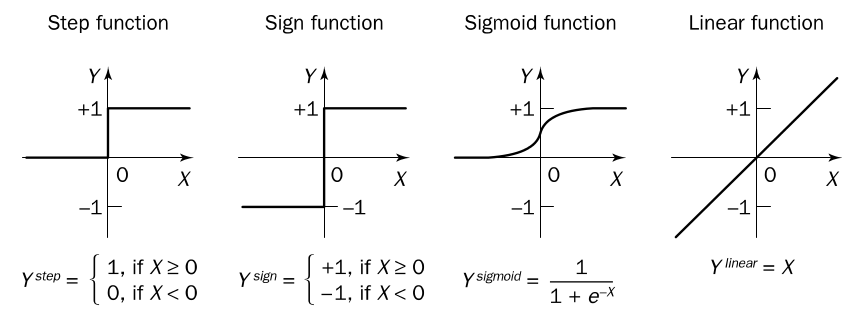
\includegraphics[scale=0.28]{factores/screen3.png}
    \caption{Normalizando f3}
  \end{subfigure}
  ~
  \begin{subfigure}[b]{.45\textwidth}
    
\includegraphics[scale=0.28]{factores/screen4.png}
    \caption{Reduciendo y marginalizando}
  \end{subfigure}
  \caption{Ejecución del código solución: crea dos factores, los multiplica, normaliza, reduce y marginaliza}
  \label{fig:P5solution}
\end{figure}

No olviden documentar y comentar su código.
